\\documentclass{article}
\usepackage{amsmath}
\usepackage{amssymb}
\usepackage{graphicx}
\usepackage[spanish]{babel}
\usepackage[utf8]{inputenc}
\begin{document}

\title{TAREA 3 - Métodos Computacionales}
\author{Daniel Ávila \\  201530842 - 201533119  \\ \textit{Universidad de los Andes. Bogotá, Colombia}}
\maketitle


%Secciones 
\section{Ecuación de onda en 2 dimensiones}
Se soluciono la ecuación de onda en dos dimensiones $$\frac{1}{c^2}\frac{\partial^2\psi(\vec r,t)}{\partial t^2}= \frac{\partial^2\psi(\vec r,x)}{\partial x^2} + \frac{\partial^2\psi(\vec r,y)}{\partial y^2}$$ 

para el caso de un estanque con una barrera. Para esto se implementó un método de \textit{diferencias finitas}; con ello se realizó la discretización de la ecuación diferencial. Asimismo, se tuvieron en cuenta una serie de condiciones iniciales y de frontera –en este caso cerradas– para solucionar la ecuación.

A continuación se exhiben los resultados de dicha simulación para los tiempos $t=30$  y $t=60$:

\begin{figure}[h!]
\centering
\includegraphics[scale=0.45]{grafica_o_1.png}
\caption{Estado de la ecuación de onda para el tiempo $t_{30}$}
\end{figure}

\begin{figure}[h!]
\centering
\includegraphics[scale=0.45]{grafica_o_1.png}
\caption{Estado de la ecuación de onda para el tiempo $t_{60}$}
\end{figure}

\section{Sistema solar}
El objetivo de este punto era simular la evolución temporal y espacial de las orbitas presentes en el sistema solar. Estuvimos previstos de unos valores iniciales de posición y velocidad para cada planeta, con lo cual se resolvió la ecuación de movimiento para cada planeta durante un intervalo de tiempo de 250 años (aproximadamente el tiempo que tarda Plutón en barrer completamente su orbita). Hubo que implementar Leap-Frog para solucionar dicha ecuación; salvaguardando el principio de conservación de la energía. 

A continuación se muestran las orbitas de los planetas.

\begin{figure}[h!]
\centering
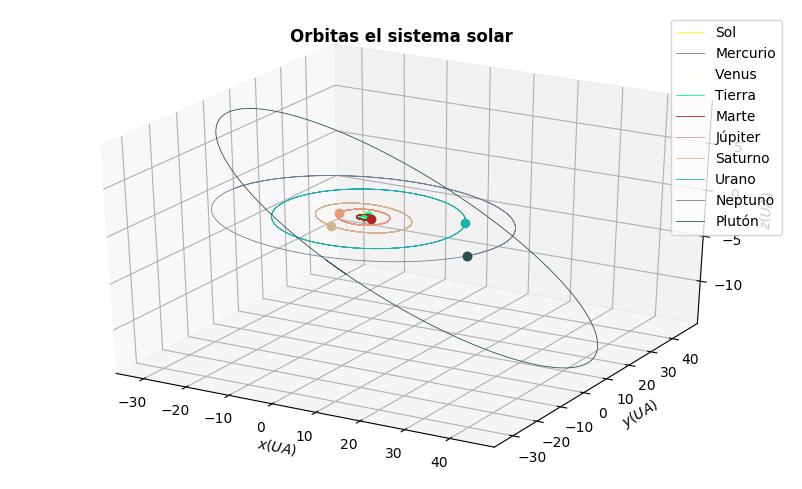
\includegraphics[scale=0.45]{grafica_p_1.png}
\caption{Orbitas en el sistema solar}
\end{figure}


\end{document}